\documentclass[conference,a4paper]{IEEEtran}

\usepackage{iftex}
\ifXeTeX
  \usepackage{newtxmath}
  \usepackage{fontspec}
  \setmainfont{texgyretermes}[Extension=.otf, UprightFont=*-regular,
    BoldFont=*-bold, ItalicFont=*-italic, BoldItalicFont=*-bolditalic]
\else
  \usepackage[utf8]{inputenc}
  \usepackage[T1]{fontenc}
  \usepackage{newtxtext,newtxmath}
\fi
\usepackage[brazil]{babel}
\usepackage{graphicx}
\usepackage{float}
\usepackage{booktabs}
\usepackage{multirow}
\usepackage{array}
\usepackage{cite}
\usepackage{url}
\usepackage[hidelinks]{hyperref}

\graphicspath{{figuras/}{../docs/figuras/}}
\renewcommand{\IEEEkeywordsname}{Palavras-chave}
\raggedbottom

\begin{document}

\title{Transferência de Aprendizagem com ResNet18 para Classificação de Uso e Cobertura do Solo na Base EuroSAT}

\author{\IEEEauthorblockN{Matheus Carneiro (RA 23003891), Guilherme Medeiros (RA 23000786),\\
Kauan Barbutti de Faria (RA 21006951), Gabriel Geraldo Mazolli (RA 23011007),\\
João Vitor de Athayde Abram (RA 23005120), Murilo de Souza Freitas (RA 23012056),\\
Integrante 7 (RA 00000000)}
\IEEEauthorblockA{Engenharia da Computação\\
Pontifícia Universidade Católica de Campinas (PUC-Campinas)\\
Campinas, SP, Brasil}}

\maketitle

\begin{abstract}
Este trabalho avalia o uso de transferência de aprendizagem para classificar imagens de satélite da base EuroSAT RGB em dez classes de uso e cobertura do solo. Partimos de uma ResNet18 pré-treinada no ImageNet e comparamos dois experimentos sobre a mesma divisão fixa dos dados: no primeiro, apenas a camada final é treinada; no segundo, o último bloco convolucional também é ajustado. No conjunto de teste, com 4.050 imagens, o primeiro experimento chegou a 92,91\% de acurácia e 92,62\% de F1 macro. O ajuste fino elevou esses valores para 97,43\% e 97,34\%, reduzindo o número de erros de 287 para 104. Os maiores ganhos ocorreram nas classes \textit{Highway}, \textit{River} e \textit{PermanentCrop}, que dependem de padrões de textura e forma pouco comuns no ImageNet. A análise dos erros restantes mostra que a maior parte envolve estruturas lineares (rodovias e rios) e áreas de cultivo semelhantes entre si.
\end{abstract}

\begin{IEEEkeywords}
transferência de aprendizagem, ajuste fino, ResNet18, EuroSAT, sensoriamento remoto, classificação de imagens.
\end{IEEEkeywords}

\section{Introdução}

A classificação de uso e cobertura do solo a partir de imagens de satélite é usada em monitoramento ambiental, planejamento urbano e agricultura. Com a disponibilidade gratuita das imagens do programa Copernicus, em especial do satélite Sentinel-2~\cite{drusch2012sentinel}, tornou-se viável montar bases rotuladas grandes o suficiente para treinar redes neurais convolucionais~\cite{cheng2017remote}.

Treinar uma rede profunda do zero, porém, exige muitos dados e tempo de processamento. Uma alternativa é a transferência de aprendizagem~\cite{pan2010survey}: reaproveitar uma rede treinada em outra tarefa, como a classificação do ImageNet~\cite{deng2009imagenet}, e adaptá-la ao novo problema. Os filtros das primeiras camadas de uma rede convolucional tendem a ser genéricos (bordas, cores, texturas simples), enquanto os das últimas camadas são mais específicos da tarefa original~\cite{yosinski2014transferable}. Isso sugere duas formas de adaptação: manter toda a rede congelada e treinar só um novo classificador, ou liberar também as camadas mais profundas para que se ajustem ao novo domínio.

O objetivo deste trabalho é comparar essas duas estratégias usando a ResNet18~\cite{he2016deep} e a base EuroSAT RGB~\cite{helber2019eurosat}. Os dois experimentos usam exatamente a mesma divisão dos dados, o mesmo pré-processamento e as mesmas métricas, de modo que a diferença de desempenho possa ser atribuída à quantidade de camadas ajustadas. O escopo é o de um projeto de graduação: adaptamos um modelo existente, sem propor uma arquitetura nova.

O restante do texto está organizado assim: a Seção~\ref{sec:base} define o problema e descreve a base de dados; a Seção~\ref{sec:referencia} apresenta a ResNet18, que serve como modelo de referência, e os resultados já publicados na EuroSAT; a Seção~\ref{sec:metodo} descreve o modelo proposto, com o pré-processamento e os dois experimentos; a Seção~\ref{sec:resultados} traz os resultados, a análise dos erros e as limitações; e a Seção~\ref{sec:conclusao} conclui o trabalho.

\section{Problema e Conjunto de Dados}
\label{sec:base}

O problema tratado é de classificação multiclasse: dada uma imagem RGB de uma pequena área da superfície, vista por satélite, o modelo deve indicar qual das dez classes de uso e cobertura do solo melhor a descreve. Cada imagem tem um único rótulo. O desempenho é medido principalmente pela acurácia e pelo F1 macro em um conjunto de teste separado, que não participa de nenhuma etapa do treinamento.

A EuroSAT RGB contém 27.000 imagens de $64\times64$ pixels, recortadas de cenas do Sentinel-2 com resolução espacial de 10~m por pixel~\cite{helber2019eurosat}. Cada imagem cobre cerca de $640\times640$~m e pertence a uma de dez classes: \textit{AnnualCrop}, \textit{Forest}, \textit{HerbaceousVegetation}, \textit{Highway}, \textit{Industrial}, \textit{Pasture}, \textit{PermanentCrop}, \textit{Residential}, \textit{River} e \textit{SeaLake}. A base é levemente desbalanceada: cinco classes têm 3.000 imagens, quatro têm 2.500 e \textit{Pasture} tem 2.000.

Antes de dividir os dados, todas as imagens foram abertas com a biblioteca Pillow para verificar se havia arquivos corrompidos; nenhum foi encontrado. A divisão foi feita por amostragem estratificada. Nesse tipo de amostragem, as imagens são primeiro agrupadas por classe (os estratos), e o sorteio é feito separadamente dentro de cada grupo, sempre com a mesma proporção: 70\% de cada classe para treino, 15\% para validação e 15\% para teste, com semente fixa (42). Dessa forma, as três partições mantêm a mesma distribuição de classes da base completa. Em um sorteio simples sobre as 27.000 imagens, a quantidade de cada classe em cada partição dependeria do acaso, e uma classe poderia ficar sub-representada no teste, o que é mais provável para a menor delas e distorceria as métricas por classe. O resultado foi salvo em um arquivo JSON versionado no repositório, e todos os experimentos leem esse mesmo arquivo, sem novos sorteios. A Tabela~\ref{tab:divisao} resume as quantidades.

\begin{table}[H]
\centering
\caption{Divisão estratificada da base EuroSAT RGB}
\label{tab:divisao}
\begin{tabular}{lrrrr}
\toprule
Classe & Total & Treino & Valid. & Teste \\
\midrule
AnnualCrop           & 3.000 & 2.100 & 450 & 450 \\
Forest               & 3.000 & 2.100 & 450 & 450 \\
HerbaceousVegetation & 3.000 & 2.100 & 450 & 450 \\
Highway              & 2.500 & 1.750 & 375 & 375 \\
Industrial           & 2.500 & 1.750 & 375 & 375 \\
Pasture              & 2.000 & 1.400 & 300 & 300 \\
PermanentCrop        & 2.500 & 1.750 & 375 & 375 \\
Residential          & 3.000 & 2.100 & 450 & 450 \\
River                & 2.500 & 1.750 & 375 & 375 \\
SeaLake              & 3.000 & 2.100 & 450 & 450 \\
\midrule
Total                & 27.000 & 18.900 & 4.050 & 4.050 \\
\bottomrule
\end{tabular}
\end{table}

A estratificação garante que mesmo a classe menor (\textit{Pasture}) tenha 300 imagens no teste, o que torna mais confiável o cálculo do F1 macro e da matriz de confusão.

\section{Sobre o Modelo de Referência}
\label{sec:referencia}

\subsection{ResNet18}

O modelo de referência deste trabalho é a ResNet18~\cite{he2016deep}, uma rede convolucional da família das redes residuais. A principal ideia da ResNet é o bloco residual: em vez de aprender diretamente uma transformação $H(x)$, cada bloco aprende uma correção $F(x)$ que é somada à própria entrada,
\begin{equation}
y = F(x) + x .
\end{equation}
Essa ligação direta facilita a passagem do gradiente durante o treino e permitiu treinar redes bem mais profundas do que as anteriores sem perda de desempenho.

A ResNet18 tem cerca de 11,2 milhões de parâmetros, organizados em uma camada convolucional inicial com \textit{max pooling}, quatro estágios de blocos residuais (\texttt{layer1} a \texttt{layer4}), cada um com dois blocos, uma média global (\textit{global average pooling}) e uma camada totalmente conectada (\texttt{fc}) com 1.000 saídas. A cada estágio, a resolução espacial cai pela metade e o número de canais dobra, de 64 até 512. Usamos a implementação da biblioteca Torchvision~\cite{torchvision2016}, com os pesos \texttt{IMAGENET1K\_V1}, obtidos no treinamento da rede para as 1.000 classes do ImageNet~\cite{deng2009imagenet}. A escolha da ResNet18, e não de versões maiores, se deve ao seu tamanho reduzido, que torna viável o treino em CPU.

\subsection{Resultados de referência na EuroSAT}

Cheng \textit{et al.}~\cite{cheng2017remote} revisaram bases e métodos para classificação de cenas em sensoriamento remoto e mostraram que redes convolucionais pré-treinadas superam com folga os descritores manuais tradicionais. Helber \textit{et al.}~\cite{helber2018introducing,helber2019eurosat} apresentaram a EuroSAT, construída com imagens do Sentinel-2, e avaliaram redes como GoogLeNet e ResNet-50 com transferência de aprendizagem a partir do ImageNet. No trabalho original, a ResNet-50 ajustada nas bandas RGB atingiu 98,57\% de acurácia, com divisão de 80\% para treino e 20\% para teste.

Yosinski \textit{et al.}~\cite{yosinski2014transferable} quantificaram o quanto as camadas de uma rede são transferíveis e observaram que ajustar as camadas transferidas melhora o resultado mesmo quando a tarefa de origem é bem diferente da de destino. Kornblith \textit{et al.}~\cite{kornblith2019better} mostraram que, em várias bases, o ajuste fino costuma superar o uso da rede apenas como extratora de características. Este trabalho segue essa linha, mas com uma rede menor (ResNet18) e um orçamento de treino reduzido, compatível com execução em CPU.

\section{Modelo Proposto}
\label{sec:metodo}

O modelo proposto consiste em adaptar a ResNet18 pré-treinada à EuroSAT, trocando sua camada de saída e treinando a rede em duas configurações: na primeira, só a nova camada de saída é ajustada; na segunda, o último estágio de blocos residuais também é ajustado. As duas configurações usam o mesmo pré-processamento, a mesma divisão dos dados e as mesmas métricas.

\subsection{Pré-processamento}

As imagens foram ampliadas de $64\times64$ para $224\times224$ pixels, resolução usada no pré-treino da ResNet18, com a transformação \texttt{Resize} da Torchvision. Essa transformação usa interpolação bilinear: cada pixel da imagem ampliada é calculado como uma média ponderada dos quatro pixels mais próximos da imagem original, o que produz uma imagem suavizada, sem os blocos que surgiriam se cada pixel fosse simplesmente repetido. Com a entrada original, o mapa de características ao fim da última camada convolucional teria apenas $2\times2$ posições, contra $7\times7$ com 224 pixels. A ampliação não acrescenta informação, mas deixa os objetos em uma escala mais próxima daquela que os filtros pré-treinados reconhecem.

Em seguida, com os pixels já convertidos para a escala de 0 a 1, cada canal $c$ (R, G e B) foi normalizado por
\begin{equation}
x'_c = \frac{x_c - \mu_c}{\sigma_c},
\end{equation}
em que $\mu_c$ e $\sigma_c$ são a média e o desvio padrão daquele canal calculados sobre as imagens de treino do ImageNet: $\mu = (0{,}485;\, 0{,}456;\, 0{,}406)$ e $\sigma = (0{,}229;\, 0{,}224;\, 0{,}225)$. A ResNet18 foi pré-treinada com entradas normalizadas exatamente dessa forma, então usar os mesmos valores mantém as imagens da EuroSAT na escala que os pesos pré-treinados esperam. Isso é especialmente importante no Experimento 1, em que quase toda a rede fica congelada.

Somente no treino, foi aplicado aumento de dados (\textit{data augmentation}), isto é, variações aleatórias que geram versões diferentes de cada imagem a cada época, sem mudar sua classe: espelhamentos horizontal e vertical, rotações em múltiplos de $90^\circ$ e uma variação leve de brilho, contraste e saturação ($\pm10\%$), sem alterar o matiz. Como as imagens de satélite são vistas de cima, não existe um lado certo para cima, e as rotações de $90^\circ$ não criam bordas vazias. Recortes aleatórios não foram usados porque, em imagens tão pequenas, poderiam remover justamente o elemento que define a classe (uma estrada ou um rio, por exemplo). A Fig.~\ref{fig:aumentos} mostra uma imagem original e cinco versões aumentadas. Validação e teste recebem apenas o redimensionamento e a normalização, sem aumento de dados, de modo que cada imagem gera sempre o mesmo tensor e os dois experimentos são avaliados sobre entradas idênticas.

\begin{figure}[H]
\centering
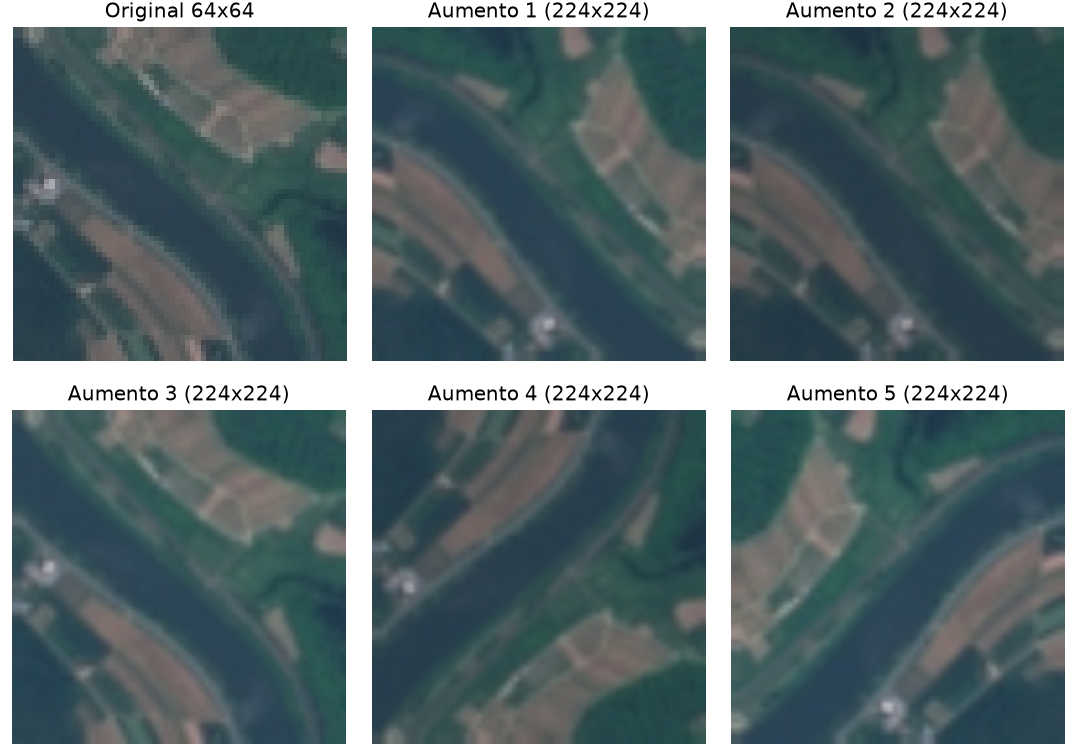
\includegraphics[width=0.75\columnwidth]{aumentos_grade.png}
\caption{Imagem original da classe \textit{River} ($64\times64$) e cinco variações geradas no treino, já em $224\times224$.}
\label{fig:aumentos}
\end{figure}

O conjunto de treino é embaralhado a cada época, com semente fixa, e os lotes têm 64 imagens. Isso é necessário porque o arquivo de divisão está ordenado por classe: sem o embaralhamento, cada lote teria uma única classe.

\subsection{Adaptação da camada de saída}

A camada \texttt{fc} original, com 1.000 saídas, foi substituída por uma nova camada linear com 512 entradas e 10 saídas, uma por classe, inicializada aleatoriamente. O restante da rede mantém os pesos do ImageNet. Todo o código foi escrito em Python com PyTorch~\cite{paszke2019pytorch}.

\subsection{Experimento 1: treino da camada final}

No primeiro experimento, todos os pesos da rede original ficam congelados e só a nova camada \texttt{fc} é treinada, o que corresponde a 5.130 parâmetros. As camadas de \textit{batch normalization}~\cite{ioffe2015batch} também permanecem em modo de avaliação, para que suas médias e variâncias não sejam alteradas pelos lotes da EuroSAT. Nesse cenário, a rede funciona como uma extratora fixa de características e o treino ajusta apenas um classificador linear sobre elas.

O treino durou 3 épocas, com otimizador Adam~\cite{kingma2015adam}, taxa de aprendizado de $10^{-3}$ e função de perda de entropia cruzada. Ao fim de cada época, o modelo é avaliado na validação, e é salvo aquele com maior acurácia de validação.

\subsection{Experimento 2: ajuste fino do último bloco}

No segundo experimento, o bloco \texttt{layer4} também é liberado para treino, além da camada \texttt{fc}. Isso eleva o número de parâmetros treináveis para 8.398.858, ou 75,11\% da rede, já que o último bloco concentra a maior parte dos pesos. As camadas iniciais (\texttt{conv1} a \texttt{layer3}) e suas estatísticas de \textit{batch normalization} continuam congeladas, preservando os filtros mais genéricos.

O treino parte do melhor modelo do Experimento 1 (\textit{warm start}), e não diretamente dos pesos do ImageNet. Assim, a nova camada \texttt{fc} já começa ajustada e não envia gradientes aleatórios para o bloco recém-liberado. Foram usadas 5 épocas, otimizador Adam com taxa de aprendizado menor ($10^{-4}$), para não destruir rapidamente o que foi aprendido no pré-treino, e o mesmo critério de seleção pela validação.

\subsection{Métricas}

Os dois modelos selecionados foram avaliados uma única vez no conjunto de teste, que não foi usado em nenhuma decisão de treino. Foram calculadas a acurácia, o F1 macro (média simples do F1 das dez classes, que dá o mesmo peso a classes com menos imagens), a precisão, a revocação e o F1 de cada classe, além da matriz de confusão~\cite{sokolova2009systematic,pedregosa2011scikit}. Para verificar se a diferença entre os modelos é estatisticamente significativa, aplicamos o teste de McNemar~\cite{mcnemar1947note} às predições pareadas das 4.050 imagens de teste. Esse teste foi escolhido porque os dois modelos são avaliados sobre as mesmas imagens, então seus resultados não são independentes, e comparar as duas acurácias como se viessem de amostras diferentes não seria adequado. O McNemar considera apenas as imagens em que os modelos discordam, isto é, em que um acerta e o outro erra, e verifica se essas discordâncias estão equilibradas, como se esperaria caso os dois modelos tivessem o mesmo desempenho.

\subsection{Ambiente de execução}

O código escolhe o dispositivo automaticamente: usa a GPU, por meio do CUDA, quando há uma disponível e, caso contrário, executa na CPU. As execuções registradas neste trabalho foram feitas em CPU, no Windows, com 8 \textit{threads}. O Experimento 1 foi executado com o PyTorch 2.14.1, e o Experimento 2 e a avaliação, com o PyTorch 2.15.0. Cada época do Experimento 1 levou cerca de 4,6 minutos; as do Experimento 2 levaram entre 10,6 e 15,1 minutos, totalizando cerca de 67,5 minutos. Os gráficos foram gerados com a Matplotlib~\cite{hunter2007matplotlib}.

\section{Resultados}
\label{sec:resultados}

\subsection{Treinamento e validação}

A Tabela~\ref{tab:treino} mostra a evolução dos dois experimentos na validação. No Experimento 1, a perda caiu nas três épocas e a melhor acurácia de validação foi de 93,36\%, na época 3. A acurácia de treino ficou abaixo da de validação, o que é esperado: ela é calculada sobre imagens com variações aleatórias e acumulada ao longo da época, enquanto o modelo ainda está mudando. A Fig.~\ref{fig:curva_inicial} mostra as curvas correspondentes.

\begin{table}[H]
\centering
\caption{Perda e acurácia por época nos dois experimentos}
\label{tab:treino}
\begin{tabular}{cccccc}
\toprule
Exp. & Época & \multicolumn{2}{c}{Treino} & \multicolumn{2}{c}{Validação} \\
\cmidrule(lr){3-4}\cmidrule(lr){5-6}
 & & Perda & Acur. (\%) & Perda & Acur. (\%) \\
\midrule
\multirow{3}{*}{1} & 1 & 0,6087 & 85,37 & 0,3004 & 91,56 \\
                   & 2 & 0,2746 & 91,82 & 0,2318 & 93,06 \\
                   & 3 & 0,2303 & 92,79 & 0,2095 & \textbf{93,36} \\
\midrule
\multirow{5}{*}{2} & 1 & 0,2069 & 93,62 & 0,1239 & 95,98 \\
                   & 2 & 0,1038 & 96,50 & 0,1002 & 96,91 \\
                   & 3 & 0,0787 & 97,23 & 0,0900 & 97,16 \\
                   & 4 & 0,0655 & 97,77 & 0,0782 & \textbf{97,63} \\
                   & 5 & 0,0539 & 98,17 & 0,0925 & 97,41 \\
\bottomrule
\end{tabular}
\end{table}

\begin{figure}[H]
\centering
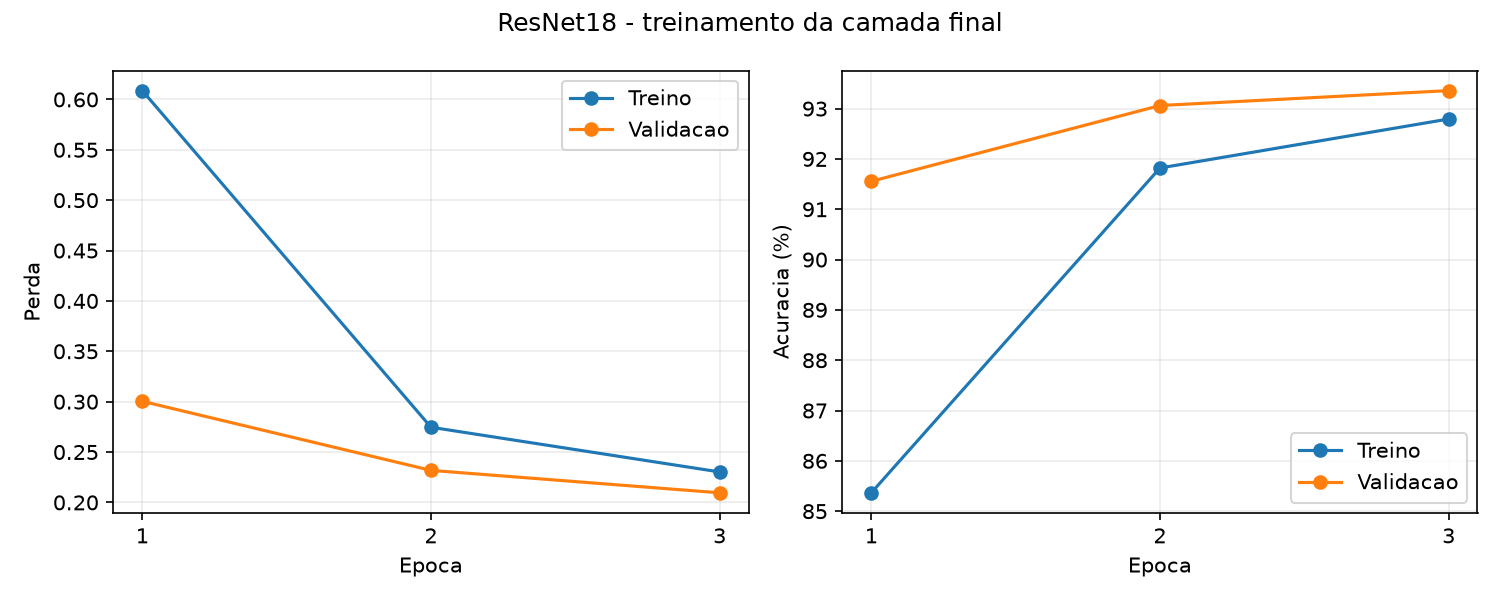
\includegraphics[width=0.94\columnwidth]{treinamento_inicial.png}
\caption{Perda e acurácia por época no Experimento 1 (apenas a camada final).}
\label{fig:curva_inicial}
\end{figure}

No Experimento 2, a acurácia de validação passou de 93,31\% (valor do modelo usado como ponto de partida\footnote{O modelo de partida foi obtido em uma nova execução do Experimento 1, com o mesmo código e as mesmas configurações; sua acurácia de validação ficou 0,05 ponto percentual abaixo da registrada na Tabela~\ref{tab:treino}.}) para 95,98\% já na primeira época. O melhor resultado foi na época 4, com 97,63\%. Na época 5, a perda de treino continuou caindo, mas a perda de validação subiu de 0,0782 para 0,0925 e a acurácia recuou para 97,41\%, um primeiro sinal de sobreajuste (Fig.~\ref{fig:curva_fino}). Como o modelo salvo é sempre o de melhor validação, essa última época foi descartada.

\begin{figure}[H]
\centering
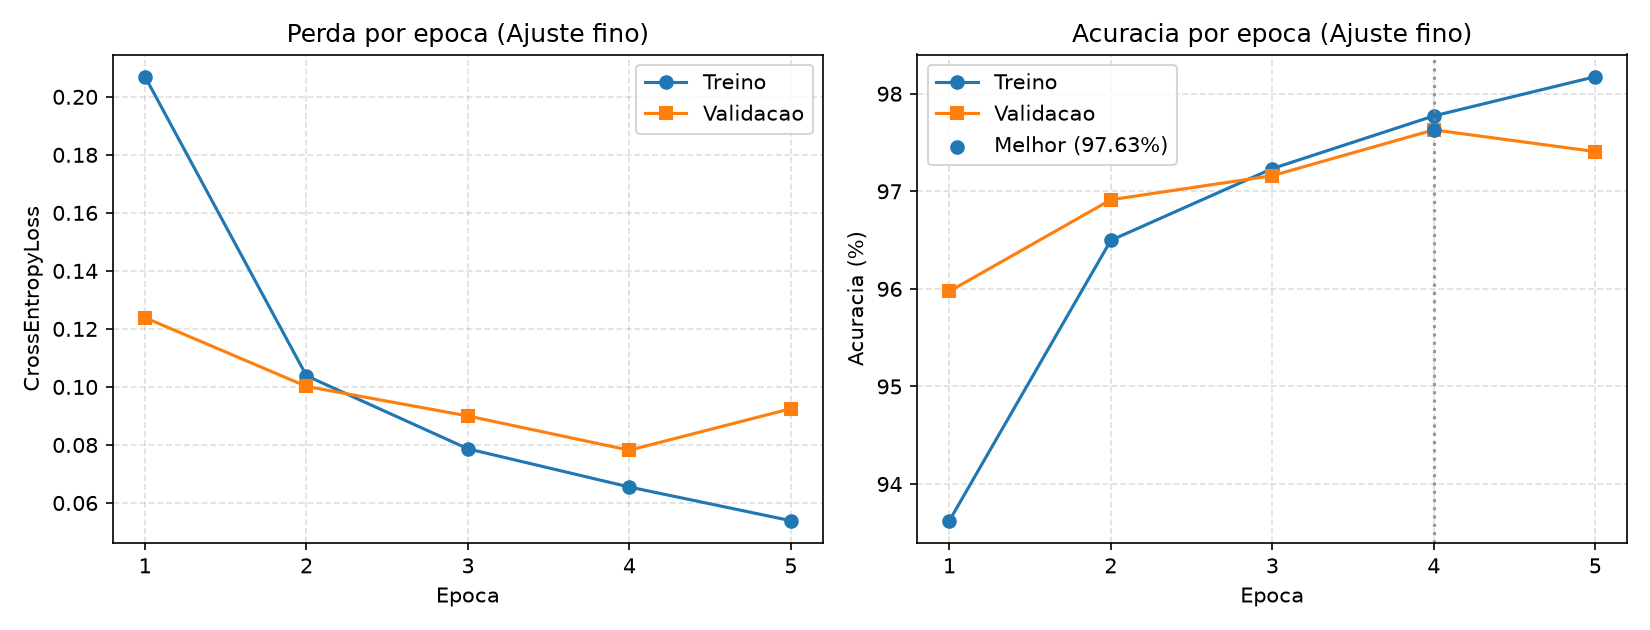
\includegraphics[width=0.94\columnwidth]{ajuste_fino.png}
\caption{Perda e acurácia por época no Experimento 2 (\texttt{layer4} + \texttt{fc}). A linha pontilhada marca a época selecionada.}
\label{fig:curva_fino}
\end{figure}

\subsection{Comparação no conjunto de teste}

A Tabela~\ref{tab:teste} resume o desempenho no teste. O ajuste fino aumentou a acurácia em 4,52 pontos percentuais e o F1 macro em 4,72 pontos, e o número de erros caiu de 287 para 104, uma redução de 63,8\%. Os valores de teste ficaram próximos dos de validação da Tabela~\ref{tab:treino} nos dois casos (diferenças de 0,45 e 0,20 ponto percentual), o que indica que a seleção de modelos pela validação não favoreceu indevidamente nenhum dos experimentos.

\begin{table}[H]
\centering
\caption{Desempenho no conjunto de teste (4.050 imagens)}
\label{tab:teste}
\begin{tabular}{lcccc}
\toprule
Experimento & Acur. (\%) & F1 macro (\%) & Acertos & Erros \\
\midrule
1 -- \texttt{fc}            & 92,91 & 92,62 & 3.763 & 287 \\
2 -- \texttt{layer4}+\texttt{fc} & \textbf{97,43} & \textbf{97,34} & \textbf{3.946} & \textbf{104} \\
\midrule
Diferença                   & +4,52 & +4,72 & +183 & $-$183 \\
\bottomrule
\end{tabular}
\end{table}

Na comparação imagem a imagem, 215 imagens erradas pelo Experimento 1 passaram a ser classificadas corretamente após o ajuste fino, 32 imagens que estavam corretas passaram a ser erradas e 72 continuaram erradas nos dois modelos. Com esses números, o teste de McNemar com correção de continuidade resulta em
\begin{equation}
\chi^2 = \frac{(|215 - 32| - 1)^2}{215 + 32} \approx 134{,}1,
\label{eq:mcnemar}
\end{equation}
com um grau de liberdade, o que corresponde a $p < 0{,}001$. A diferença entre os dois modelos, portanto, não pode ser explicada por variação aleatória nas imagens de teste.

A Tabela~\ref{tab:classes} detalha o desempenho por classe, e a Fig.~\ref{fig:comparacao} compara visualmente o F1 de cada classe. Todas as classes melhoraram com o ajuste fino, e todas passaram a ter F1 acima de 94,8\%. Os maiores ganhos foram em \textit{PermanentCrop} (+7,70 pontos), \textit{River} (+7,62) e \textit{Highway} (+7,44), justamente as classes com pior desempenho no Experimento 1. Nesse experimento, \textit{Highway} e \textit{PermanentCrop} tinham revocação de apenas 82,1\% e 82,4\%, ou seja, quase uma em cada cinco imagens dessas classes era atribuída a outra classe. Com o ajuste fino, as revocações subiram para 95,2\% e 95,5\%.

\begin{table}[H]
\centering
\caption{Precisão (P), revocação (R) e F1 por classe no conjunto de teste, em porcentagem}
\label{tab:classes}
\setlength{\tabcolsep}{3pt}
\resizebox{\columnwidth}{!}{%
\begin{tabular}{lccccccc}
\toprule
\multirow{2}{*}{Classe} & \multicolumn{3}{c}{Exp. 1 (\texttt{fc})} & \multicolumn{3}{c}{Exp. 2 (\texttt{layer4}+\texttt{fc})} & \multirow{2}{*}{Ganho F1} \\
\cmidrule(lr){2-4}\cmidrule(lr){5-7}
 & P & R & F1 & P & R & F1 & \\
\midrule
AnnualCrop           & 94,05 & 94,89 & 94,47 & 98,42 & 96,89 & 97,65 & +3,18 \\
Forest               & 92,89 & 98,67 & 95,69 & 98,67 & 99,11 & 98,89 & +3,20 \\
HerbaceousVegetation & 92,20 & 92,00 & 92,10 & 96,46 & 96,89 & 96,67 & +4,57 \\
Highway              & 93,33 & 82,13 & 87,38 & 94,44 & 95,20 & 94,82 & +7,44 \\
Industrial           & 91,07 & 97,87 & 94,34 & 99,18 & 96,53 & 97,84 & +3,49 \\
Pasture              & 90,16 & 94,67 & 92,36 & 96,70 & 97,67 & 97,18 & +4,82 \\
PermanentCrop        & 95,67 & 82,40 & 88,54 & 97,02 & 95,47 & 96,24 & +7,70 \\
Residential          & 94,04 & 98,22 & 96,09 & 98,89 & 99,33 & 99,11 & +3,03 \\
River                & 86,04 & 90,40 & 88,17 & 94,55 & 97,07 & 95,79 & +7,62 \\
SeaLake              & 98,85 & 95,33 & 97,06 & 99,11 & 99,33 & 99,22 & +2,16 \\
\midrule
Média (macro)        & -- & -- & 92,62 & -- & -- & 97,34 & +4,72 \\
\bottomrule
\end{tabular}}
\end{table}

\begin{figure}[H]
\centering
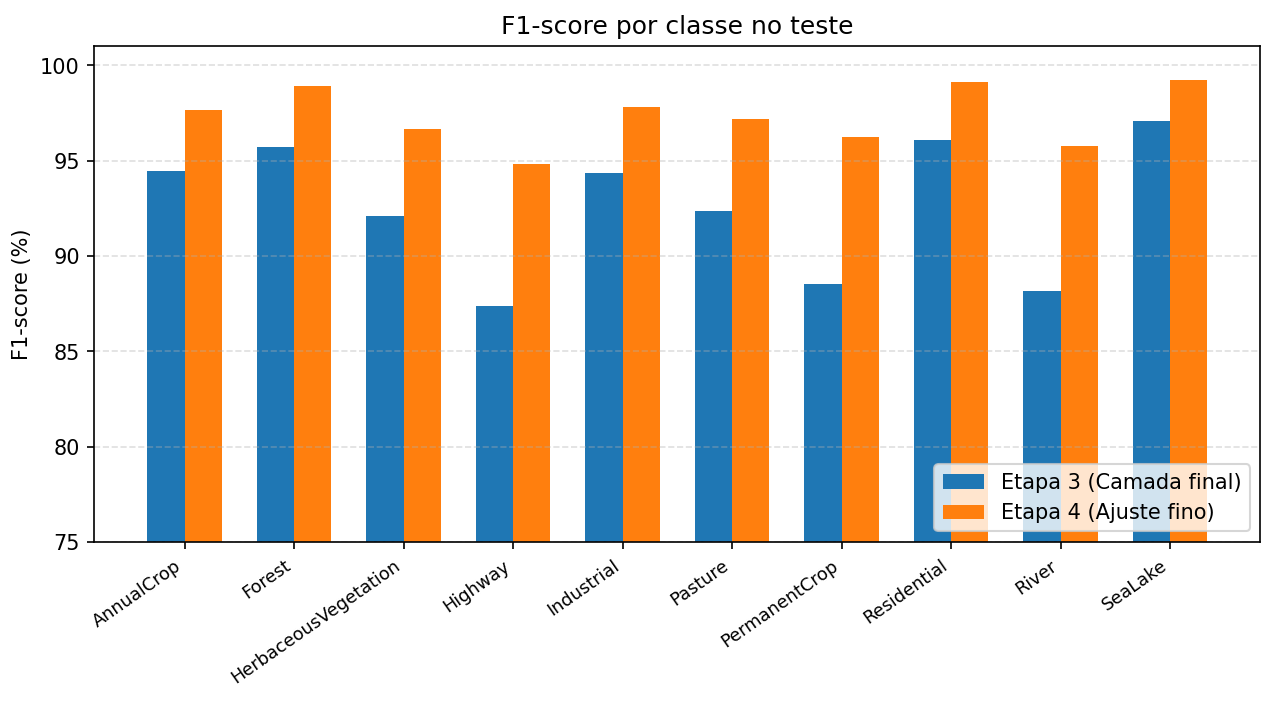
\includegraphics[width=\columnwidth]{comparacao_classes.png}
\caption{F1 por classe no conjunto de teste para os dois experimentos. No gráfico, ``Etapa 3'' corresponde ao Experimento 1 e ``Etapa 4'', ao Experimento 2.}
\label{fig:comparacao}
\end{figure}

\subsection{Matrizes de confusão}

As matrizes de confusão das Figs.~\ref{fig:matriz1} e~\ref{fig:matriz2} mostram onde os erros se concentram. No Experimento 1, as confusões mais frequentes foram entre classes que, vistas de cima, têm aparência parecida: 28 imagens de \textit{Highway} foram classificadas como \textit{River}, ambas formadas por uma faixa estreita e alongada atravessando outra cobertura; 20 imagens de \textit{PermanentCrop} foram classificadas como \textit{HerbaceousVegetation} e 12 como \textit{AnnualCrop}; e 14 imagens de \textit{HerbaceousVegetation} foram classificadas como \textit{Forest}.

\begin{figure}[H]
\centering
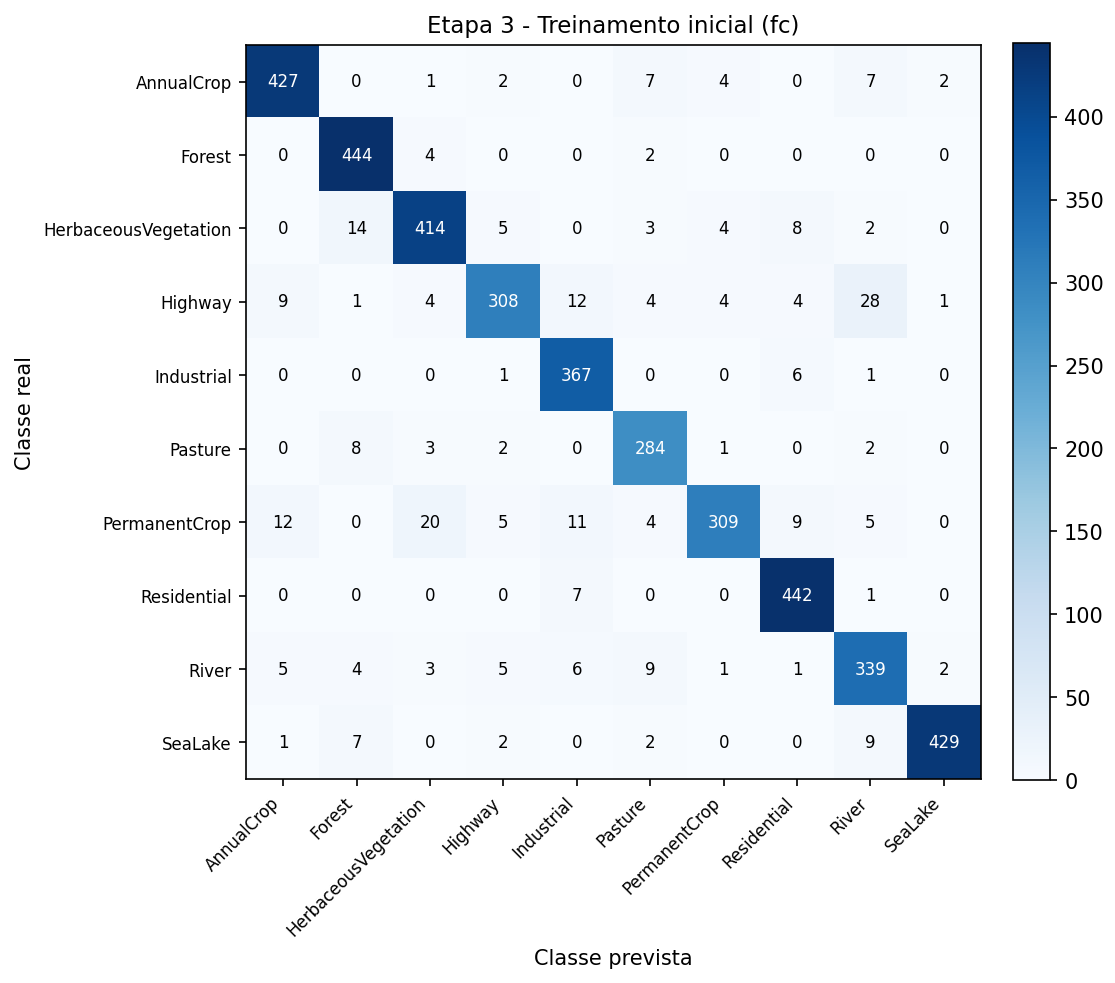
\includegraphics[width=0.8\columnwidth]{matriz_exp1.png}
\caption{Matriz de confusão do Experimento 1 (apenas \texttt{fc}) no conjunto de teste. As linhas indicam a classe real e as colunas, a classe prevista.}
\label{fig:matriz1}
\end{figure}

Após o ajuste fino (Fig.~\ref{fig:matriz2}), essas confusões diminuíram bastante: \textit{Highway}$\rightarrow$\textit{River} caiu de 28 para 11 casos, \textit{PermanentCrop}$\rightarrow$\textit{HerbaceousVegetation} de 20 para 9 e \textit{HerbaceousVegetation}$\rightarrow$\textit{Forest} de 14 para 1. A interpretação é que os filtros do \texttt{layer4}, originalmente ajustados para objetos do ImageNet, passaram a responder a padrões próprios das imagens de satélite, como a largura e a textura de uma faixa linear ou o espaçamento regular das fileiras de um cultivo permanente. Com a rede congelada, o classificador linear só podia combinar características que não foram aprendidas para separar esses casos.

\begin{figure}[H]
\centering
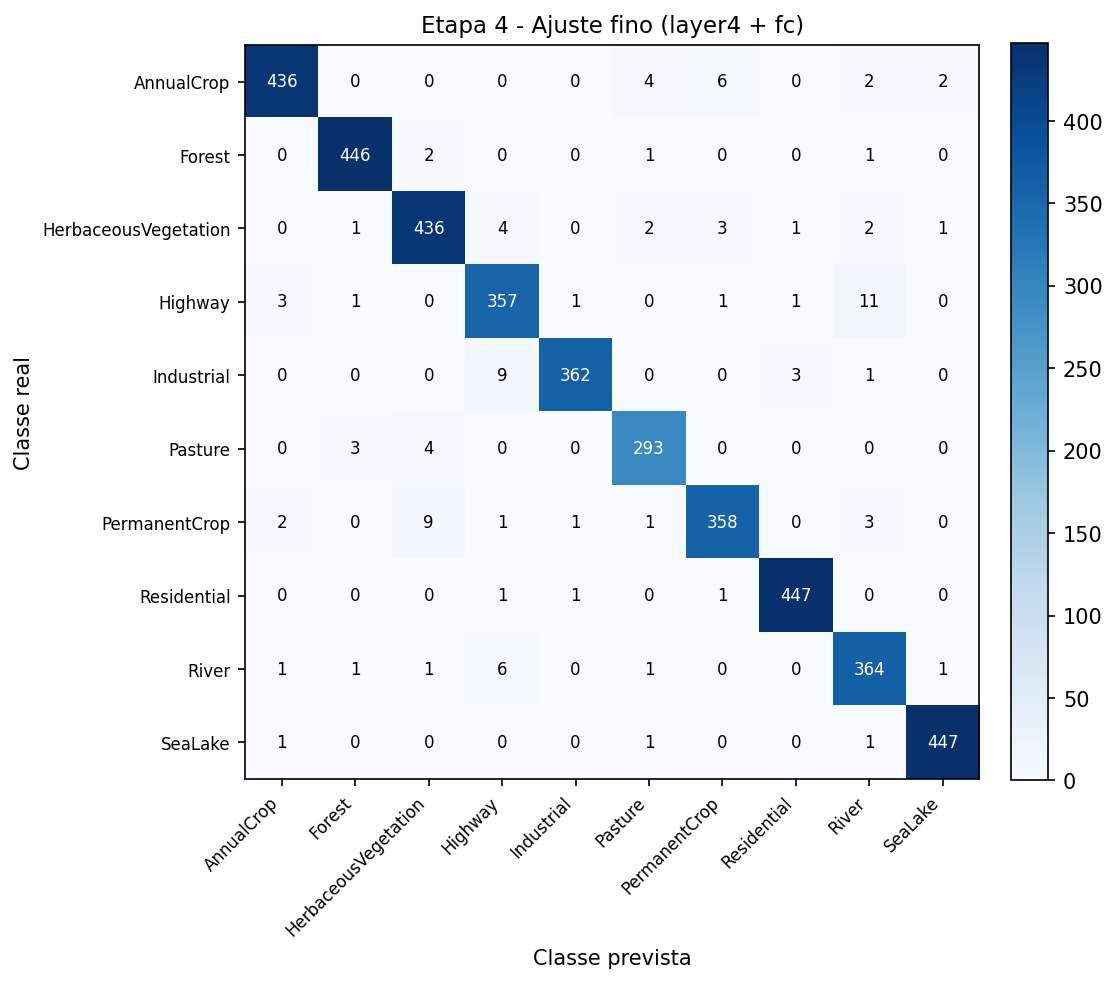
\includegraphics[width=0.8\columnwidth]{matriz_exp2.png}
\caption{Matriz de confusão do Experimento 2 (\texttt{layer4} + \texttt{fc}) no conjunto de teste.}
\label{fig:matriz2}
\end{figure}

\subsection{Análise dos erros}

Dos 104 erros que restaram no Experimento 2 (Tabela~\ref{tab:teste}), a maior parte envolve estruturas lineares, como mostra a Fig.~\ref{fig:matriz2}: são 17 confusões entre \textit{Highway} e \textit{River} nos dois sentidos, além de 9 imagens de \textit{Industrial} classificadas como \textit{Highway}. Outro grupo envolve as classes de vegetação e cultivo (\textit{PermanentCrop}, \textit{HerbaceousVegetation} e \textit{AnnualCrop}). A Fig.~\ref{fig:erros} mostra os nove erros com maior confiança do modelo.

\begin{figure}[H]
\centering
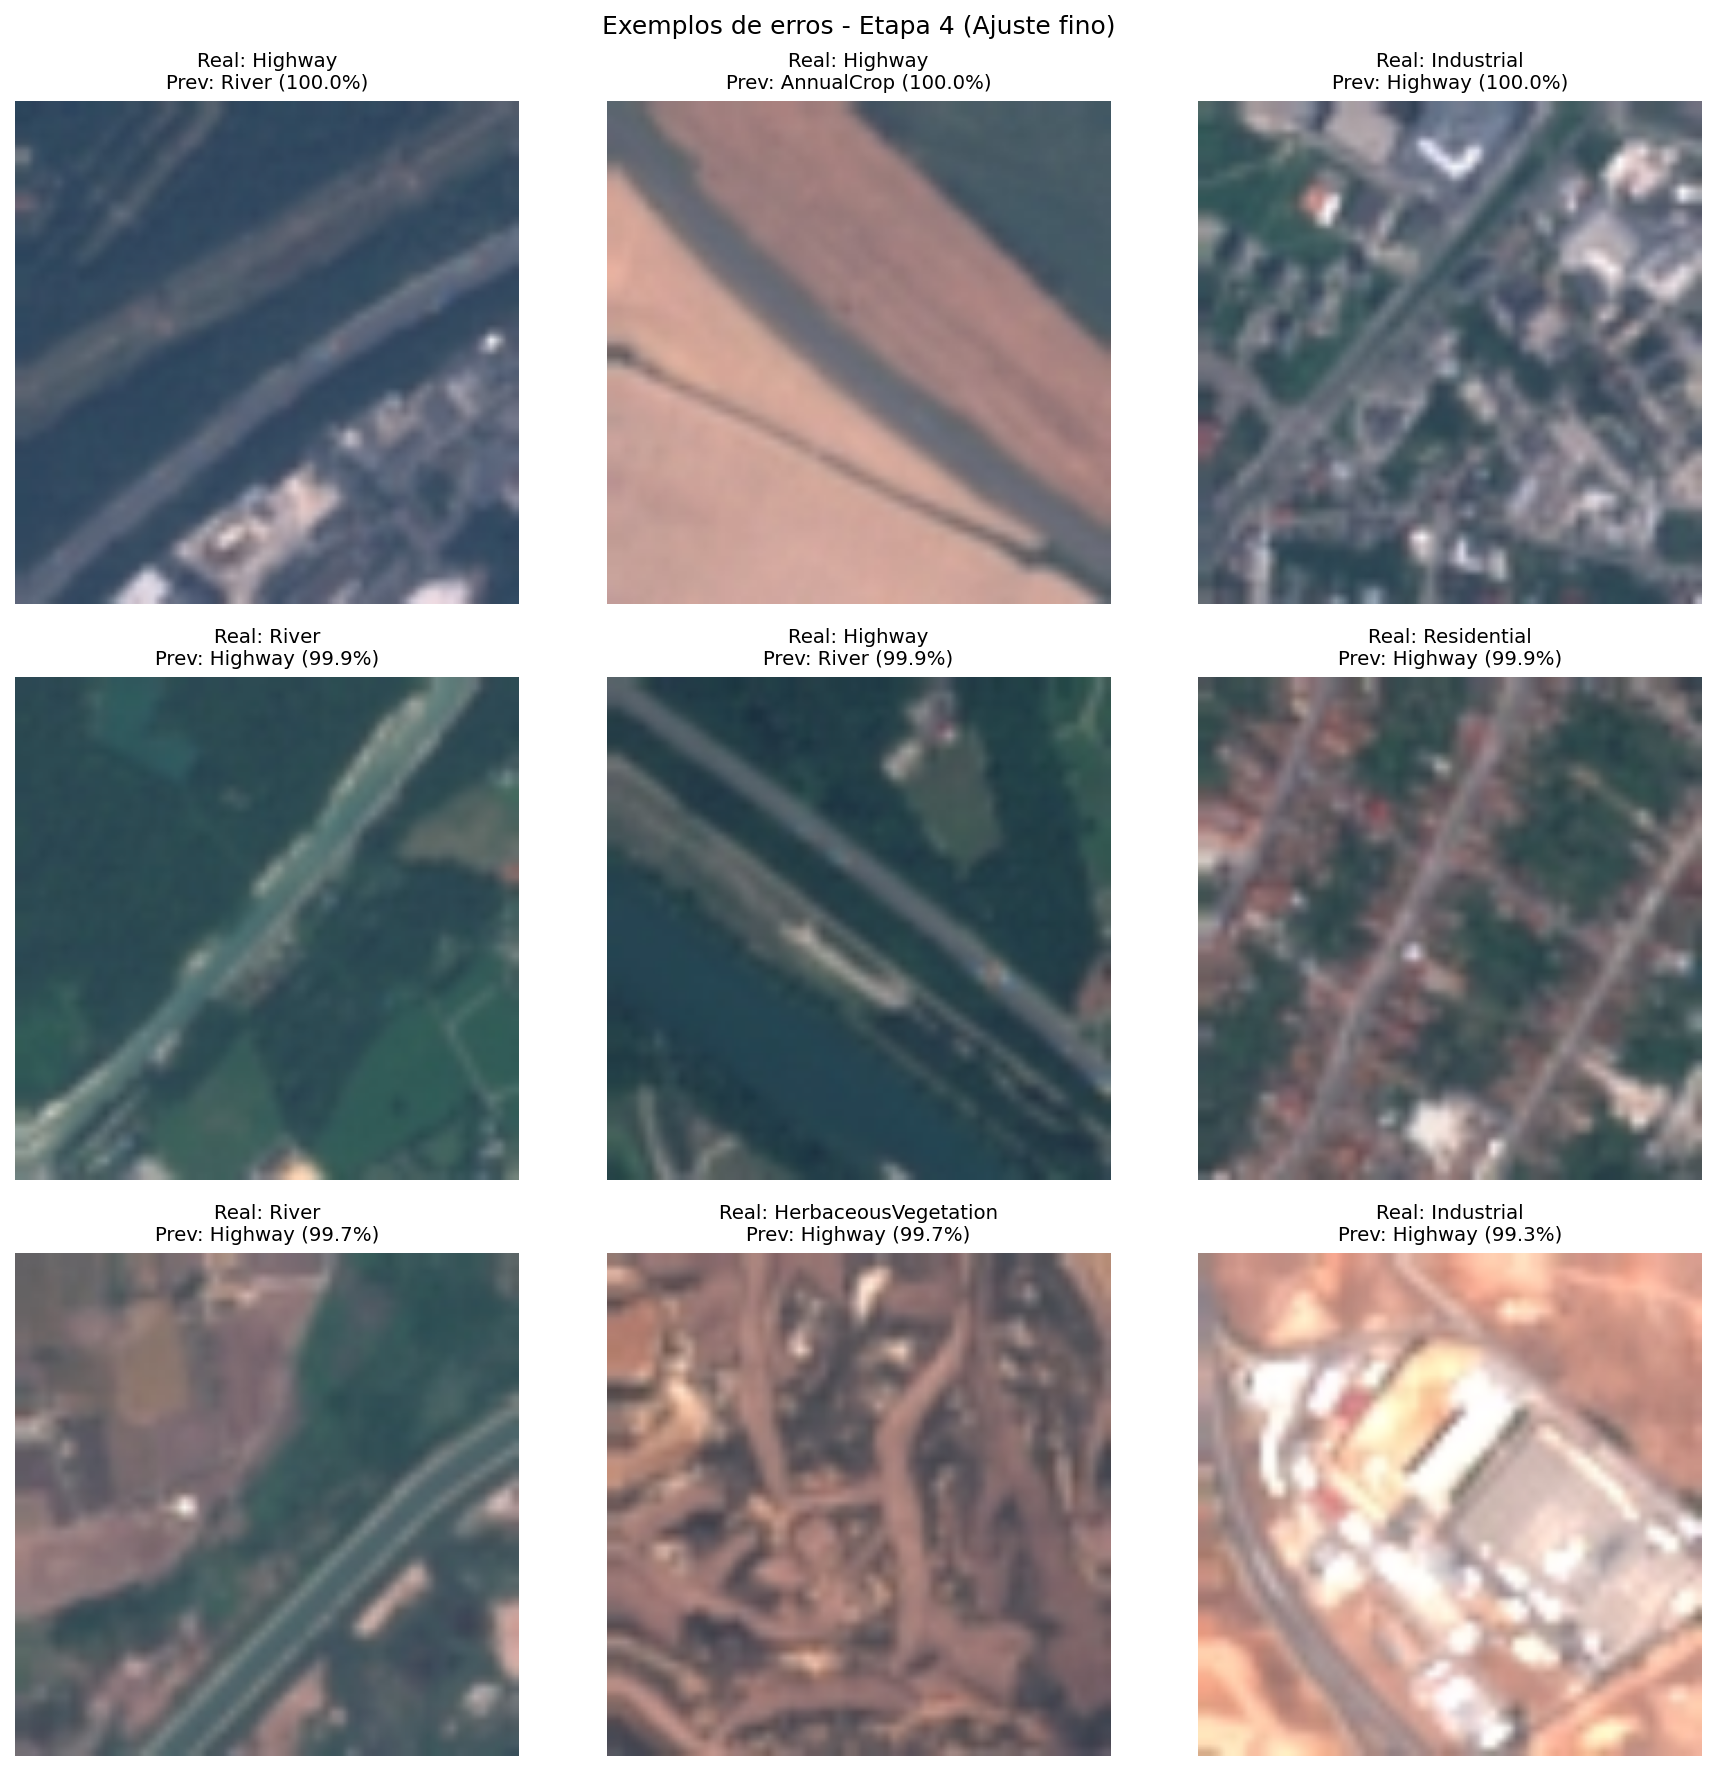
\includegraphics[width=0.66\columnwidth]{exemplos_erros_ajuste_fino.png}
\caption{Os nove erros de maior confiança do Experimento 2, com a classe real e a classe prevista.}
\label{fig:erros}
\end{figure}

Observando essas imagens, nota-se que vários erros não são equívocos grosseiros do modelo. Em muitas delas há mais de uma classe presente no mesmo recorte: áreas industriais e residenciais cortadas por vias largas, ou uma rodovia que corre ao lado de um rio. Como cada imagem tem um único rótulo e cobre uma área pequena, o elemento que define a classe às vezes ocupa uma parte menor do quadro do que outro elemento que o modelo reconhece com segurança. Em alguns casos, como imagens rotuladas como \textit{River} em que se vê com clareza uma rodovia, o rótulo da própria base parece questionável. O fato de esses erros terem confiança acima de 99\% reforça que o modelo está reagindo a um conteúdo real da imagem. Também se observa que imagens como \textit{Highway\_848} e \textit{Highway\_891} foram erradas pelos dois modelos, o que sugere que são casos intrinsecamente ambíguos, e não falhas de um treinamento específico.

\subsection{Discussão e limitações}
\label{sec:discussao}

Os resultados confirmam o que a literatura aponta~\cite{yosinski2014transferable,kornblith2019better}: os filtros pré-treinados no ImageNet já são úteis para imagens de satélite, a ponto de um classificador linear sobre eles atingir quase 93\% de acurácia (Tabela~\ref{tab:teste}), mas ajustar as camadas mais profundas ao novo domínio traz um ganho grande. A distância entre o ImageNet (fotos de objetos tiradas no nível do chão) e a EuroSAT (vista aérea, sem orientação definida) ajuda a explicar por que as camadas mais específicas precisam ser adaptadas. O resultado de 97,43\% (Tabela~\ref{tab:teste}) ficou próximo dos 98,57\% relatados por Helber \textit{et al.}~\cite{helber2019eurosat} com a ResNet-50, uma rede maior, com divisão de dados diferente e mais tempo de treino.

Algumas limitações devem ser consideradas. Primeiro, os dois experimentos não tiveram o mesmo número de épocas: o Experimento 2 parte do modelo do Experimento 1 e treina por mais 5 épocas, totalizando 8. Parte do ganho pode vir apenas do treino mais longo, embora as curvas do Experimento 1 já mostrem que a acurácia de validação estava se estabilizando. Segundo, os números de épocas e as taxas de aprendizado foram escolhidos para manter o tempo de execução viável em CPU, sem busca de hiperparâmetros. Terceiro, cada experimento foi executado com uma única semente, então não temos uma estimativa da variação entre execuções; o teste de McNemar avalia a variação devida às imagens de teste, mas não a do treinamento. Por fim, foram usadas apenas as bandas RGB, enquanto o Sentinel-2 fornece 13 bandas espectrais que podem ajudar a separar tipos de vegetação.

Como trabalhos futuros, seria interessante liberar mais blocos da rede (por exemplo, \texttt{layer3}), comparar com um ajuste fino partindo diretamente dos pesos do ImageNet, repetir os experimentos com várias sementes e usar GPU para treinar por mais épocas.

\section{Conclusão}
\label{sec:conclusao}

Este trabalho comparou duas formas de adaptar a ResNet18 pré-treinada no ImageNet para classificar a EuroSAT RGB. Treinar apenas a camada final resultou em 92,91\% de acurácia no teste (Tabela~\ref{tab:teste}), um resultado razoável dado que apenas 5.130 parâmetros foram ajustados. Liberar também o último bloco convolucional elevou a acurácia para 97,43\% e o F1 macro para 97,34\%, com melhora em todas as dez classes (Tabela~\ref{tab:classes} e Fig.~\ref{fig:comparacao}) e redução de 63,8\% no número de erros. A diferença é estatisticamente significativa segundo o teste de McNemar (Eq.~\ref{eq:mcnemar}). Os erros restantes (Figs.~\ref{fig:matriz2} e~\ref{fig:erros}) se concentram em imagens que misturam mais de uma classe ou cuja classe é difícil de distinguir na resolução de $64\times64$ pixels.

Todo o código, a divisão fixa dos dados, os históricos de treinamento e os resultados da avaliação estão disponíveis no repositório do projeto\footnote{\url{https://github.com/GabrielGM3/Projeto-Visao-computacional}}, o que permite reproduzir os experimentos e a comparação.

\section*{Divisão do Trabalho}

O projeto foi dividido em sete funções: (1) obtenção e divisão da base de dados; (2) preparação das imagens; (3) adaptação da ResNet18 e treinamento da camada final; (4) ajuste fino do último bloco; (5) avaliação e análise dos resultados; (6) redação do relatório e organização das referências; e (7) apresentação e instruções de reprodução. Cada integrante ficou responsável por uma função e todos participaram da revisão do fluxo completo.

\bibliographystyle{IEEEtran}
\bibliography{referencias}

\end{document}
